% Created by tikzDevice version 0.12.6 on 2026-02-13 15:17:01
% !TEX encoding = UTF-8 Unicode
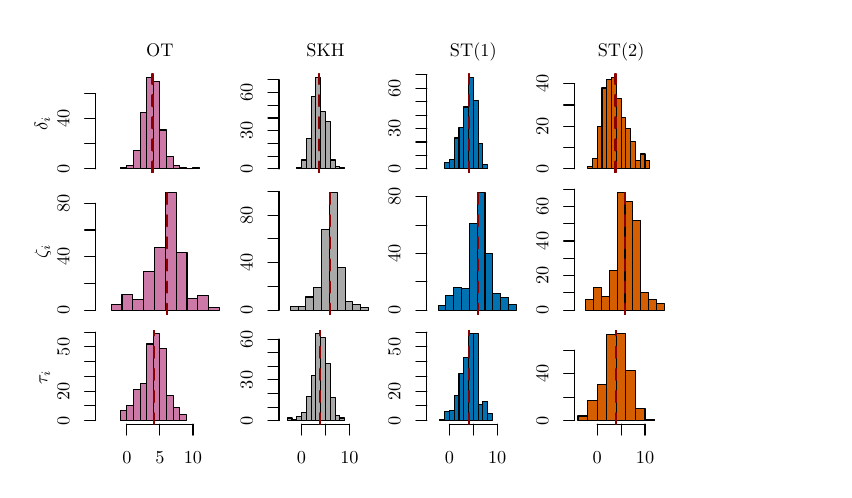
\begin{tikzpicture}[x=1pt,y=1pt]
\definecolor{fillColor}{RGB}{255,255,255}
\path[use as bounding box,fill=fillColor,fill opacity=0.00] (0,0) rectangle (287.82,159.90);
\begin{scope}
\path[clip] ( 24.55,107.54) rectangle ( 71.01,143.27);
\definecolor{drawColor}{RGB}{0,0,0}
\definecolor{fillColor}{RGB}{204,121,167}

\path[draw=drawColor,line width= 0.4pt,line join=round,line cap=round,fill=fillColor] ( 33.44,108.87) rectangle ( 35.83,109.32);

\path[draw=drawColor,line width= 0.4pt,line join=round,line cap=round,fill=fillColor] ( 35.83,108.87) rectangle ( 38.22,110.23);

\path[draw=drawColor,line width= 0.4pt,line join=round,line cap=round,fill=fillColor] ( 38.22,108.87) rectangle ( 40.61,115.66);

\path[draw=drawColor,line width= 0.4pt,line join=round,line cap=round,fill=fillColor] ( 40.61,108.87) rectangle ( 43.00,129.26);

\path[draw=drawColor,line width= 0.4pt,line join=round,line cap=round,fill=fillColor] ( 43.00,108.87) rectangle ( 45.39,141.94);

\path[draw=drawColor,line width= 0.4pt,line join=round,line cap=round,fill=fillColor] ( 45.39,108.87) rectangle ( 47.78,140.58);

\path[draw=drawColor,line width= 0.4pt,line join=round,line cap=round,fill=fillColor] ( 47.78,108.87) rectangle ( 50.17,122.91);

\path[draw=drawColor,line width= 0.4pt,line join=round,line cap=round,fill=fillColor] ( 50.17,108.87) rectangle ( 52.56,113.40);

\path[draw=drawColor,line width= 0.4pt,line join=round,line cap=round,fill=fillColor] ( 52.56,108.87) rectangle ( 54.95,110.23);

\path[draw=drawColor,line width= 0.4pt,line join=round,line cap=round,fill=fillColor] ( 54.95,108.87) rectangle ( 57.34,109.32);

\path[draw=drawColor,line width= 0.4pt,line join=round,line cap=round,fill=fillColor] ( 57.34,108.87) rectangle ( 59.73,108.87);

\path[draw=drawColor,line width= 0.4pt,line join=round,line cap=round,fill=fillColor] ( 59.73,108.87) rectangle ( 62.12,109.32);
\end{scope}
\begin{scope}
\path[clip] (  0.00,  0.00) rectangle (287.82,159.90);
\definecolor{drawColor}{RGB}{0,0,0}

\path[draw=drawColor,line width= 0.4pt,line join=round,line cap=round] ( 24.55,108.87) -- ( 24.55,136.05);

\path[draw=drawColor,line width= 0.4pt,line join=round,line cap=round] ( 24.55,108.87) -- ( 20.59,108.87);

\path[draw=drawColor,line width= 0.4pt,line join=round,line cap=round] ( 24.55,117.93) -- ( 20.59,117.93);

\path[draw=drawColor,line width= 0.4pt,line join=round,line cap=round] ( 24.55,126.99) -- ( 20.59,126.99);

\path[draw=drawColor,line width= 0.4pt,line join=round,line cap=round] ( 24.55,136.05) -- ( 20.59,136.05);

\node[text=drawColor,rotate= 90.00,anchor=base,inner sep=0pt, outer sep=0pt, scale=  0.66] at ( 15.05,108.87) {0};

\node[text=drawColor,rotate= 90.00,anchor=base,inner sep=0pt, outer sep=0pt, scale=  0.66] at ( 15.05,126.99) {40};
\end{scope}
\begin{scope}
\path[clip] (  0.00,102.79) rectangle ( 74.18,159.90);
\definecolor{drawColor}{RGB}{0,0,0}

\node[text=drawColor,anchor=base,inner sep=0pt, outer sep=0pt, scale=  0.66] at ( 47.78,149.31) {OT};

\node[text=drawColor,rotate= 90.00,anchor=base,inner sep=0pt, outer sep=0pt, scale=  0.66] at (  7.13,125.40) {$\delta_i$};
\end{scope}
\begin{scope}
\path[clip] ( 24.55,107.54) rectangle ( 71.01,143.27);
\definecolor{drawColor}{RGB}{139,0,0}

\path[draw=drawColor,line width= 0.8pt,dash pattern=on 4pt off 4pt ,line join=round,line cap=round] ( 45.12,107.54) -- ( 45.12,143.27);
\end{scope}
\begin{scope}
\path[clip] ( 24.55, 56.15) rectangle ( 71.01,102.00);
\definecolor{drawColor}{RGB}{0,0,0}
\definecolor{fillColor}{RGB}{204,121,167}

\path[draw=drawColor,line width= 0.4pt,line join=round,line cap=round,fill=fillColor] ( 30.18, 57.85) rectangle ( 34.09, 59.78);

\path[draw=drawColor,line width= 0.4pt,line join=round,line cap=round,fill=fillColor] ( 34.09, 57.85) rectangle ( 38.00, 63.64);

\path[draw=drawColor,line width= 0.4pt,line join=round,line cap=round,fill=fillColor] ( 38.00, 57.85) rectangle ( 41.92, 61.71);

\path[draw=drawColor,line width= 0.4pt,line join=round,line cap=round,fill=fillColor] ( 41.92, 57.85) rectangle ( 45.83, 71.84);

\path[draw=drawColor,line width= 0.4pt,line join=round,line cap=round,fill=fillColor] ( 45.83, 57.85) rectangle ( 49.74, 80.52);

\path[draw=drawColor,line width= 0.4pt,line join=round,line cap=round,fill=fillColor] ( 49.74, 57.85) rectangle ( 53.65,100.30);

\path[draw=drawColor,line width= 0.4pt,line join=round,line cap=round,fill=fillColor] ( 53.65, 57.85) rectangle ( 57.56, 78.59);

\path[draw=drawColor,line width= 0.4pt,line join=round,line cap=round,fill=fillColor] ( 57.56, 57.85) rectangle ( 61.47, 62.19);

\path[draw=drawColor,line width= 0.4pt,line join=round,line cap=round,fill=fillColor] ( 61.47, 57.85) rectangle ( 65.38, 63.15);

\path[draw=drawColor,line width= 0.4pt,line join=round,line cap=round,fill=fillColor] ( 65.38, 57.85) rectangle ( 69.29, 58.81);
\end{scope}
\begin{scope}
\path[clip] (  0.00,  0.00) rectangle (287.82,159.90);
\definecolor{drawColor}{RGB}{0,0,0}

\path[draw=drawColor,line width= 0.4pt,line join=round,line cap=round] ( 24.55, 57.85) -- ( 24.55, 96.44);

\path[draw=drawColor,line width= 0.4pt,line join=round,line cap=round] ( 24.55, 57.85) -- ( 20.59, 57.85);

\path[draw=drawColor,line width= 0.4pt,line join=round,line cap=round] ( 24.55, 67.49) -- ( 20.59, 67.49);

\path[draw=drawColor,line width= 0.4pt,line join=round,line cap=round] ( 24.55, 77.14) -- ( 20.59, 77.14);

\path[draw=drawColor,line width= 0.4pt,line join=round,line cap=round] ( 24.55, 86.79) -- ( 20.59, 86.79);

\path[draw=drawColor,line width= 0.4pt,line join=round,line cap=round] ( 24.55, 96.44) -- ( 20.59, 96.44);

\node[text=drawColor,rotate= 90.00,anchor=base,inner sep=0pt, outer sep=0pt, scale=  0.66] at ( 15.05, 57.85) {0};

\node[text=drawColor,rotate= 90.00,anchor=base,inner sep=0pt, outer sep=0pt, scale=  0.66] at ( 15.05, 77.14) {40};

\node[text=drawColor,rotate= 90.00,anchor=base,inner sep=0pt, outer sep=0pt, scale=  0.66] at ( 15.05, 96.44) {80};
\end{scope}
\begin{scope}
\path[clip] (  0.00, 51.40) rectangle ( 74.18,102.79);
\definecolor{drawColor}{RGB}{0,0,0}

\node[text=drawColor,rotate= 90.00,anchor=base,inner sep=0pt, outer sep=0pt, scale=  0.66] at (  7.13, 79.07) {$\zeta_i$};
\end{scope}
\begin{scope}
\path[clip] ( 24.55, 56.15) rectangle ( 71.01,102.00);
\definecolor{drawColor}{RGB}{139,0,0}

\path[draw=drawColor,line width= 0.8pt,dash pattern=on 4pt off 4pt ,line join=round,line cap=round] ( 50.34, 56.15) -- ( 50.34,102.00);
\end{scope}
\begin{scope}
\path[clip] ( 24.55, 16.63) rectangle ( 71.01, 50.60);
\definecolor{drawColor}{RGB}{0,0,0}
\definecolor{fillColor}{RGB}{204,121,167}

\path[draw=drawColor,line width= 0.4pt,line join=round,line cap=round,fill=fillColor] ( 33.44, 17.89) rectangle ( 35.83, 21.62);

\path[draw=drawColor,line width= 0.4pt,line join=round,line cap=round,fill=fillColor] ( 35.83, 17.89) rectangle ( 38.22, 23.22);

\path[draw=drawColor,line width= 0.4pt,line join=round,line cap=round,fill=fillColor] ( 38.22, 17.89) rectangle ( 40.61, 29.09);

\path[draw=drawColor,line width= 0.4pt,line join=round,line cap=round,fill=fillColor] ( 40.61, 17.89) rectangle ( 43.00, 31.22);

\path[draw=drawColor,line width= 0.4pt,line join=round,line cap=round,fill=fillColor] ( 43.00, 17.89) rectangle ( 45.39, 45.61);

\path[draw=drawColor,line width= 0.4pt,line join=round,line cap=round,fill=fillColor] ( 45.39, 17.89) rectangle ( 47.78, 49.35);

\path[draw=drawColor,line width= 0.4pt,line join=round,line cap=round,fill=fillColor] ( 47.78, 17.89) rectangle ( 50.17, 44.01);

\path[draw=drawColor,line width= 0.4pt,line join=round,line cap=round,fill=fillColor] ( 50.17, 17.89) rectangle ( 52.56, 26.95);

\path[draw=drawColor,line width= 0.4pt,line join=round,line cap=round,fill=fillColor] ( 52.56, 17.89) rectangle ( 54.95, 22.69);

\path[draw=drawColor,line width= 0.4pt,line join=round,line cap=round,fill=fillColor] ( 54.95, 17.89) rectangle ( 57.34, 20.02);
\end{scope}
\begin{scope}
\path[clip] (  0.00,  0.00) rectangle (287.82,159.90);
\definecolor{drawColor}{RGB}{0,0,0}

\path[draw=drawColor,line width= 0.4pt,line join=round,line cap=round] ( 35.83, 16.63) -- ( 59.73, 16.63);

\path[draw=drawColor,line width= 0.4pt,line join=round,line cap=round] ( 35.83, 16.63) -- ( 35.83, 12.67);

\path[draw=drawColor,line width= 0.4pt,line join=round,line cap=round] ( 47.78, 16.63) -- ( 47.78, 12.67);

\path[draw=drawColor,line width= 0.4pt,line join=round,line cap=round] ( 59.73, 16.63) -- ( 59.73, 12.67);

\node[text=drawColor,anchor=base,inner sep=0pt, outer sep=0pt, scale=  0.66] at ( 35.83,  2.38) {0};

\node[text=drawColor,anchor=base,inner sep=0pt, outer sep=0pt, scale=  0.66] at ( 47.78,  2.38) {5};

\node[text=drawColor,anchor=base,inner sep=0pt, outer sep=0pt, scale=  0.66] at ( 59.73,  2.38) {10};

\path[draw=drawColor,line width= 0.4pt,line join=round,line cap=round] ( 24.55, 17.89) -- ( 24.55, 49.88);

\path[draw=drawColor,line width= 0.4pt,line join=round,line cap=round] ( 24.55, 17.89) -- ( 20.59, 17.89);

\path[draw=drawColor,line width= 0.4pt,line join=round,line cap=round] ( 24.55, 23.22) -- ( 20.59, 23.22);

\path[draw=drawColor,line width= 0.4pt,line join=round,line cap=round] ( 24.55, 28.55) -- ( 20.59, 28.55);

\path[draw=drawColor,line width= 0.4pt,line join=round,line cap=round] ( 24.55, 33.88) -- ( 20.59, 33.88);

\path[draw=drawColor,line width= 0.4pt,line join=round,line cap=round] ( 24.55, 39.22) -- ( 20.59, 39.22);

\path[draw=drawColor,line width= 0.4pt,line join=round,line cap=round] ( 24.55, 44.55) -- ( 20.59, 44.55);

\path[draw=drawColor,line width= 0.4pt,line join=round,line cap=round] ( 24.55, 49.88) -- ( 20.59, 49.88);

\node[text=drawColor,rotate= 90.00,anchor=base,inner sep=0pt, outer sep=0pt, scale=  0.66] at ( 15.05, 17.89) {0};

\node[text=drawColor,rotate= 90.00,anchor=base,inner sep=0pt, outer sep=0pt, scale=  0.66] at ( 15.05, 28.55) {20};

\node[text=drawColor,rotate= 90.00,anchor=base,inner sep=0pt, outer sep=0pt, scale=  0.66] at ( 15.05, 44.55) {50};
\end{scope}
\begin{scope}
\path[clip] (  0.00,  0.00) rectangle ( 74.18, 51.40);
\definecolor{drawColor}{RGB}{0,0,0}

\node[text=drawColor,rotate= 90.00,anchor=base,inner sep=0pt, outer sep=0pt, scale=  0.66] at (  7.13, 33.62) {$\tau_i$};
\end{scope}
\begin{scope}
\path[clip] ( 24.55, 16.63) rectangle ( 71.01, 50.60);
\definecolor{drawColor}{RGB}{139,0,0}

\path[draw=drawColor,line width= 0.8pt,dash pattern=on 4pt off 4pt ,line join=round,line cap=round] ( 45.62, 16.63) -- ( 45.62, 50.60);
\end{scope}
\begin{scope}
\path[clip] ( 90.81,107.54) rectangle (124.42,143.27);
\definecolor{drawColor}{RGB}{0,0,0}
\definecolor{fillColor}{RGB}{169,169,169}

\path[draw=drawColor,line width= 0.4pt,line join=round,line cap=round,fill=fillColor] ( 97.24,108.87) rectangle ( 98.97,109.33);

\path[draw=drawColor,line width= 0.4pt,line join=round,line cap=round,fill=fillColor] ( 98.97,108.87) rectangle (100.70,112.08);

\path[draw=drawColor,line width= 0.4pt,line join=round,line cap=round,fill=fillColor] (100.70,108.87) rectangle (102.43,119.89);

\path[draw=drawColor,line width= 0.4pt,line join=round,line cap=round,fill=fillColor] (102.43,108.87) rectangle (104.16,135.05);

\path[draw=drawColor,line width= 0.4pt,line join=round,line cap=round,fill=fillColor] (104.16,108.87) rectangle (105.89,141.94);

\path[draw=drawColor,line width= 0.4pt,line join=round,line cap=round,fill=fillColor] (105.89,108.87) rectangle (107.62,129.54);

\path[draw=drawColor,line width= 0.4pt,line join=round,line cap=round,fill=fillColor] (107.62,108.87) rectangle (109.34,125.86);

\path[draw=drawColor,line width= 0.4pt,line join=round,line cap=round,fill=fillColor] (109.34,108.87) rectangle (111.07,112.08);

\path[draw=drawColor,line width= 0.4pt,line join=round,line cap=round,fill=fillColor] (111.07,108.87) rectangle (112.80,109.78);

\path[draw=drawColor,line width= 0.4pt,line join=round,line cap=round,fill=fillColor] (112.80,108.87) rectangle (114.53,109.33);
\end{scope}
\begin{scope}
\path[clip] (  0.00,  0.00) rectangle (287.82,159.90);
\definecolor{drawColor}{RGB}{0,0,0}

\path[draw=drawColor,line width= 0.4pt,line join=round,line cap=round] ( 90.81,108.87) -- ( 90.81,141.02);

\path[draw=drawColor,line width= 0.4pt,line join=round,line cap=round] ( 90.81,108.87) -- ( 86.85,108.87);

\path[draw=drawColor,line width= 0.4pt,line join=round,line cap=round] ( 90.81,113.46) -- ( 86.85,113.46);

\path[draw=drawColor,line width= 0.4pt,line join=round,line cap=round] ( 90.81,118.05) -- ( 86.85,118.05);

\path[draw=drawColor,line width= 0.4pt,line join=round,line cap=round] ( 90.81,122.65) -- ( 86.85,122.65);

\path[draw=drawColor,line width= 0.4pt,line join=round,line cap=round] ( 90.81,127.24) -- ( 86.85,127.24);

\path[draw=drawColor,line width= 0.4pt,line join=round,line cap=round] ( 90.81,131.84) -- ( 86.85,131.84);

\path[draw=drawColor,line width= 0.4pt,line join=round,line cap=round] ( 90.81,136.43) -- ( 86.85,136.43);

\path[draw=drawColor,line width= 0.4pt,line join=round,line cap=round] ( 90.81,141.02) -- ( 86.85,141.02);

\node[text=drawColor,rotate= 90.00,anchor=base,inner sep=0pt, outer sep=0pt, scale=  0.66] at ( 81.31,108.87) {0};

\node[text=drawColor,rotate= 90.00,anchor=base,inner sep=0pt, outer sep=0pt, scale=  0.66] at ( 81.31,122.65) {30};

\node[text=drawColor,rotate= 90.00,anchor=base,inner sep=0pt, outer sep=0pt, scale=  0.66] at ( 81.31,136.43) {60};
\end{scope}
\begin{scope}
\path[clip] ( 74.18,102.79) rectangle (127.59,159.90);
\definecolor{drawColor}{RGB}{0,0,0}

\node[text=drawColor,anchor=base,inner sep=0pt, outer sep=0pt, scale=  0.66] at (107.62,149.31) {SKH};
\end{scope}
\begin{scope}
\path[clip] ( 90.81,107.54) rectangle (124.42,143.27);
\definecolor{drawColor}{RGB}{139,0,0}

\path[draw=drawColor,line width= 0.8pt,dash pattern=on 4pt off 4pt ,line join=round,line cap=round] (105.17,107.54) -- (105.17,143.27);
\end{scope}
\begin{scope}
\path[clip] ( 90.81, 56.15) rectangle (124.42,102.00);
\definecolor{drawColor}{RGB}{0,0,0}
\definecolor{fillColor}{RGB}{169,169,169}

\path[draw=drawColor,line width= 0.4pt,line join=round,line cap=round,fill=fillColor] ( 94.89, 57.85) rectangle ( 97.71, 59.13);

\path[draw=drawColor,line width= 0.4pt,line join=round,line cap=round,fill=fillColor] ( 97.71, 57.85) rectangle (100.54, 59.13);

\path[draw=drawColor,line width= 0.4pt,line join=round,line cap=round,fill=fillColor] (100.54, 57.85) rectangle (103.37, 62.56);

\path[draw=drawColor,line width= 0.4pt,line join=round,line cap=round,fill=fillColor] (103.37, 57.85) rectangle (106.20, 65.99);

\path[draw=drawColor,line width= 0.4pt,line join=round,line cap=round,fill=fillColor] (106.20, 57.85) rectangle (109.03, 87.01);

\path[draw=drawColor,line width= 0.4pt,line join=round,line cap=round,fill=fillColor] (109.03, 57.85) rectangle (111.86,100.30);

\path[draw=drawColor,line width= 0.4pt,line join=round,line cap=round,fill=fillColor] (111.86, 57.85) rectangle (114.69, 73.28);

\path[draw=drawColor,line width= 0.4pt,line join=round,line cap=round,fill=fillColor] (114.69, 57.85) rectangle (117.52, 60.85);

\path[draw=drawColor,line width= 0.4pt,line join=round,line cap=round,fill=fillColor] (117.52, 57.85) rectangle (120.35, 59.99);

\path[draw=drawColor,line width= 0.4pt,line join=round,line cap=round,fill=fillColor] (120.35, 57.85) rectangle (123.18, 58.70);
\end{scope}
\begin{scope}
\path[clip] (  0.00,  0.00) rectangle (287.82,159.90);
\definecolor{drawColor}{RGB}{0,0,0}

\path[draw=drawColor,line width= 0.4pt,line join=round,line cap=round] ( 90.81, 57.85) -- ( 90.81,100.73);

\path[draw=drawColor,line width= 0.4pt,line join=round,line cap=round] ( 90.81, 57.85) -- ( 86.85, 57.85);

\path[draw=drawColor,line width= 0.4pt,line join=round,line cap=round] ( 90.81, 66.42) -- ( 86.85, 66.42);

\path[draw=drawColor,line width= 0.4pt,line join=round,line cap=round] ( 90.81, 75.00) -- ( 86.85, 75.00);

\path[draw=drawColor,line width= 0.4pt,line join=round,line cap=round] ( 90.81, 83.58) -- ( 86.85, 83.58);

\path[draw=drawColor,line width= 0.4pt,line join=round,line cap=round] ( 90.81, 92.15) -- ( 86.85, 92.15);

\path[draw=drawColor,line width= 0.4pt,line join=round,line cap=round] ( 90.81,100.73) -- ( 86.85,100.73);

\node[text=drawColor,rotate= 90.00,anchor=base,inner sep=0pt, outer sep=0pt, scale=  0.66] at ( 81.31, 57.85) {0};

\node[text=drawColor,rotate= 90.00,anchor=base,inner sep=0pt, outer sep=0pt, scale=  0.66] at ( 81.31, 75.00) {40};

\node[text=drawColor,rotate= 90.00,anchor=base,inner sep=0pt, outer sep=0pt, scale=  0.66] at ( 81.31, 92.15) {80};
\end{scope}
\begin{scope}
\path[clip] ( 90.81, 56.15) rectangle (124.42,102.00);
\definecolor{drawColor}{RGB}{139,0,0}

\path[draw=drawColor,line width= 0.8pt,dash pattern=on 4pt off 4pt ,line join=round,line cap=round] (109.38, 56.15) -- (109.38,102.00);
\end{scope}
\begin{scope}
\path[clip] ( 90.81, 16.63) rectangle (124.42, 50.60);
\definecolor{drawColor}{RGB}{0,0,0}
\definecolor{fillColor}{RGB}{169,169,169}

\path[draw=drawColor,line width= 0.4pt,line join=round,line cap=round,fill=fillColor] ( 93.78, 17.89) rectangle ( 95.51, 18.87);

\path[draw=drawColor,line width= 0.4pt,line join=round,line cap=round,fill=fillColor] ( 95.51, 17.89) rectangle ( 97.24, 18.38);

\path[draw=drawColor,line width= 0.4pt,line join=round,line cap=round,fill=fillColor] ( 97.24, 17.89) rectangle ( 98.97, 19.36);

\path[draw=drawColor,line width= 0.4pt,line join=round,line cap=round,fill=fillColor] ( 98.97, 17.89) rectangle (100.70, 20.84);

\path[draw=drawColor,line width= 0.4pt,line join=round,line cap=round,fill=fillColor] (100.70, 17.89) rectangle (102.43, 26.74);

\path[draw=drawColor,line width= 0.4pt,line join=round,line cap=round,fill=fillColor] (102.43, 17.89) rectangle (104.16, 34.11);

\path[draw=drawColor,line width= 0.4pt,line join=round,line cap=round,fill=fillColor] (104.16, 17.89) rectangle (105.89, 49.35);

\path[draw=drawColor,line width= 0.4pt,line join=round,line cap=round,fill=fillColor] (105.89, 17.89) rectangle (107.62, 47.87);

\path[draw=drawColor,line width= 0.4pt,line join=round,line cap=round,fill=fillColor] (107.62, 17.89) rectangle (109.34, 38.53);

\path[draw=drawColor,line width= 0.4pt,line join=round,line cap=round,fill=fillColor] (109.34, 17.89) rectangle (111.07, 26.25);

\path[draw=drawColor,line width= 0.4pt,line join=round,line cap=round,fill=fillColor] (111.07, 17.89) rectangle (112.80, 19.86);

\path[draw=drawColor,line width= 0.4pt,line join=round,line cap=round,fill=fillColor] (112.80, 17.89) rectangle (114.53, 18.87);
\end{scope}
\begin{scope}
\path[clip] (  0.00,  0.00) rectangle (287.82,159.90);
\definecolor{drawColor}{RGB}{0,0,0}

\path[draw=drawColor,line width= 0.4pt,line join=round,line cap=round] ( 98.97, 16.63) -- (116.26, 16.63);

\path[draw=drawColor,line width= 0.4pt,line join=round,line cap=round] ( 98.97, 16.63) -- ( 98.97, 12.67);

\path[draw=drawColor,line width= 0.4pt,line join=round,line cap=round] (107.62, 16.63) -- (107.62, 12.67);

\path[draw=drawColor,line width= 0.4pt,line join=round,line cap=round] (116.26, 16.63) -- (116.26, 12.67);

\node[text=drawColor,anchor=base,inner sep=0pt, outer sep=0pt, scale=  0.66] at ( 98.97,  2.38) {0};

\node[text=drawColor,anchor=base,inner sep=0pt, outer sep=0pt, scale=  0.66] at (116.26,  2.38) {10};

\path[draw=drawColor,line width= 0.4pt,line join=round,line cap=round] ( 90.81, 17.89) -- ( 90.81, 47.38);

\path[draw=drawColor,line width= 0.4pt,line join=round,line cap=round] ( 90.81, 17.89) -- ( 86.85, 17.89);

\path[draw=drawColor,line width= 0.4pt,line join=round,line cap=round] ( 90.81, 22.81) -- ( 86.85, 22.81);

\path[draw=drawColor,line width= 0.4pt,line join=round,line cap=round] ( 90.81, 27.72) -- ( 86.85, 27.72);

\path[draw=drawColor,line width= 0.4pt,line join=round,line cap=round] ( 90.81, 32.63) -- ( 86.85, 32.63);

\path[draw=drawColor,line width= 0.4pt,line join=round,line cap=round] ( 90.81, 37.55) -- ( 86.85, 37.55);

\path[draw=drawColor,line width= 0.4pt,line join=round,line cap=round] ( 90.81, 42.46) -- ( 86.85, 42.46);

\path[draw=drawColor,line width= 0.4pt,line join=round,line cap=round] ( 90.81, 47.38) -- ( 86.85, 47.38);

\node[text=drawColor,rotate= 90.00,anchor=base,inner sep=0pt, outer sep=0pt, scale=  0.66] at ( 81.31, 17.89) {0};

\node[text=drawColor,rotate= 90.00,anchor=base,inner sep=0pt, outer sep=0pt, scale=  0.66] at ( 81.31, 32.63) {30};

\node[text=drawColor,rotate= 90.00,anchor=base,inner sep=0pt, outer sep=0pt, scale=  0.66] at ( 81.31, 47.38) {60};
\end{scope}
\begin{scope}
\path[clip] ( 90.81, 16.63) rectangle (124.42, 50.60);
\definecolor{drawColor}{RGB}{139,0,0}

\path[draw=drawColor,line width= 0.8pt,dash pattern=on 4pt off 4pt ,line join=round,line cap=round] (105.74, 16.63) -- (105.74, 50.60);
\end{scope}
\begin{scope}
\path[clip] (144.22,107.54) rectangle (177.83,143.27);
\definecolor{drawColor}{RGB}{0,0,0}
\definecolor{fillColor}{RGB}{0,114,178}

\path[draw=drawColor,line width= 0.4pt,line join=round,line cap=round,fill=fillColor] (150.65,108.87) rectangle (152.38,111.30);

\path[draw=drawColor,line width= 0.4pt,line join=round,line cap=round,fill=fillColor] (152.38,108.87) rectangle (154.11,112.27);

\path[draw=drawColor,line width= 0.4pt,line join=round,line cap=round,fill=fillColor] (154.11,108.87) rectangle (155.84,120.05);

\path[draw=drawColor,line width= 0.4pt,line join=round,line cap=round,fill=fillColor] (155.84,108.87) rectangle (157.57,123.95);

\path[draw=drawColor,line width= 0.4pt,line join=round,line cap=round,fill=fillColor] (157.57,108.87) rectangle (159.30,131.24);

\path[draw=drawColor,line width= 0.4pt,line join=round,line cap=round,fill=fillColor] (159.30,108.87) rectangle (161.02,141.94);

\path[draw=drawColor,line width= 0.4pt,line join=round,line cap=round,fill=fillColor] (161.02,108.87) rectangle (162.75,133.67);

\path[draw=drawColor,line width= 0.4pt,line join=round,line cap=round,fill=fillColor] (162.75,108.87) rectangle (164.48,118.11);

\path[draw=drawColor,line width= 0.4pt,line join=round,line cap=round,fill=fillColor] (164.48,108.87) rectangle (166.21,110.33);
\end{scope}
\begin{scope}
\path[clip] (  0.00,  0.00) rectangle (287.82,159.90);
\definecolor{drawColor}{RGB}{0,0,0}

\path[draw=drawColor,line width= 0.4pt,line join=round,line cap=round] (144.22,108.87) -- (144.22,142.92);

\path[draw=drawColor,line width= 0.4pt,line join=round,line cap=round] (144.22,108.87) -- (140.26,108.87);

\path[draw=drawColor,line width= 0.4pt,line join=round,line cap=round] (144.22,113.73) -- (140.26,113.73);

\path[draw=drawColor,line width= 0.4pt,line join=round,line cap=round] (144.22,118.59) -- (140.26,118.59);

\path[draw=drawColor,line width= 0.4pt,line join=round,line cap=round] (144.22,123.46) -- (140.26,123.46);

\path[draw=drawColor,line width= 0.4pt,line join=round,line cap=round] (144.22,128.32) -- (140.26,128.32);

\path[draw=drawColor,line width= 0.4pt,line join=round,line cap=round] (144.22,133.19) -- (140.26,133.19);

\path[draw=drawColor,line width= 0.4pt,line join=round,line cap=round] (144.22,138.05) -- (140.26,138.05);

\path[draw=drawColor,line width= 0.4pt,line join=round,line cap=round] (144.22,142.92) -- (140.26,142.92);

\node[text=drawColor,rotate= 90.00,anchor=base,inner sep=0pt, outer sep=0pt, scale=  0.66] at (134.72,108.87) {0};

\node[text=drawColor,rotate= 90.00,anchor=base,inner sep=0pt, outer sep=0pt, scale=  0.66] at (134.72,123.46) {30};

\node[text=drawColor,rotate= 90.00,anchor=base,inner sep=0pt, outer sep=0pt, scale=  0.66] at (134.72,138.05) {60};
\end{scope}
\begin{scope}
\path[clip] (127.59,102.79) rectangle (181.00,159.90);
\definecolor{drawColor}{RGB}{0,0,0}

\node[text=drawColor,anchor=base,inner sep=0pt, outer sep=0pt, scale=  0.66] at (161.02,149.31) {ST(1)};
\end{scope}
\begin{scope}
\path[clip] (144.22,107.54) rectangle (177.83,143.27);
\definecolor{drawColor}{RGB}{139,0,0}

\path[draw=drawColor,line width= 0.8pt,dash pattern=on 4pt off 4pt ,line join=round,line cap=round] (159.34,107.54) -- (159.34,143.27);
\end{scope}
\begin{scope}
\path[clip] (144.22, 56.15) rectangle (177.83,102.00);
\definecolor{drawColor}{RGB}{0,0,0}
\definecolor{fillColor}{RGB}{0,114,178}

\path[draw=drawColor,line width= 0.4pt,line join=round,line cap=round,fill=fillColor] (148.29, 57.85) rectangle (151.12, 59.38);

\path[draw=drawColor,line width= 0.4pt,line join=round,line cap=round,fill=fillColor] (151.12, 57.85) rectangle (153.95, 62.96);

\path[draw=drawColor,line width= 0.4pt,line join=round,line cap=round,fill=fillColor] (153.95, 57.85) rectangle (156.78, 66.03);

\path[draw=drawColor,line width= 0.4pt,line join=round,line cap=round,fill=fillColor] (156.78, 57.85) rectangle (159.61, 65.52);

\path[draw=drawColor,line width= 0.4pt,line join=round,line cap=round,fill=fillColor] (159.61, 57.85) rectangle (162.44, 89.05);

\path[draw=drawColor,line width= 0.4pt,line join=round,line cap=round,fill=fillColor] (162.44, 57.85) rectangle (165.27,100.30);

\path[draw=drawColor,line width= 0.4pt,line join=round,line cap=round,fill=fillColor] (165.27, 57.85) rectangle (168.10, 78.31);

\path[draw=drawColor,line width= 0.4pt,line join=round,line cap=round,fill=fillColor] (168.10, 57.85) rectangle (170.93, 63.98);

\path[draw=drawColor,line width= 0.4pt,line join=round,line cap=round,fill=fillColor] (170.93, 57.85) rectangle (173.76, 62.45);

\path[draw=drawColor,line width= 0.4pt,line join=round,line cap=round,fill=fillColor] (173.76, 57.85) rectangle (176.58, 59.89);
\end{scope}
\begin{scope}
\path[clip] (  0.00,  0.00) rectangle (287.82,159.90);
\definecolor{drawColor}{RGB}{0,0,0}

\path[draw=drawColor,line width= 0.4pt,line join=round,line cap=round] (144.22, 57.85) -- (144.22, 98.77);

\path[draw=drawColor,line width= 0.4pt,line join=round,line cap=round] (144.22, 57.85) -- (140.26, 57.85);

\path[draw=drawColor,line width= 0.4pt,line join=round,line cap=round] (144.22, 68.08) -- (140.26, 68.08);

\path[draw=drawColor,line width= 0.4pt,line join=round,line cap=round] (144.22, 78.31) -- (140.26, 78.31);

\path[draw=drawColor,line width= 0.4pt,line join=round,line cap=round] (144.22, 88.54) -- (140.26, 88.54);

\path[draw=drawColor,line width= 0.4pt,line join=round,line cap=round] (144.22, 98.77) -- (140.26, 98.77);

\node[text=drawColor,rotate= 90.00,anchor=base,inner sep=0pt, outer sep=0pt, scale=  0.66] at (134.72, 57.85) {0};

\node[text=drawColor,rotate= 90.00,anchor=base,inner sep=0pt, outer sep=0pt, scale=  0.66] at (134.72, 78.31) {40};

\node[text=drawColor,rotate= 90.00,anchor=base,inner sep=0pt, outer sep=0pt, scale=  0.66] at (134.72, 98.77) {80};
\end{scope}
\begin{scope}
\path[clip] (144.22, 56.15) rectangle (177.83,102.00);
\definecolor{drawColor}{RGB}{139,0,0}

\path[draw=drawColor,line width= 0.8pt,dash pattern=on 4pt off 4pt ,line join=round,line cap=round] (162.83, 56.15) -- (162.83,102.00);
\end{scope}
\begin{scope}
\path[clip] (144.22, 16.63) rectangle (177.83, 50.60);
\definecolor{drawColor}{RGB}{0,0,0}
\definecolor{fillColor}{RGB}{0,114,178}

\path[draw=drawColor,line width= 0.4pt,line join=round,line cap=round,fill=fillColor] (148.92, 17.89) rectangle (150.65, 18.42);

\path[draw=drawColor,line width= 0.4pt,line join=round,line cap=round,fill=fillColor] (150.65, 17.89) rectangle (152.38, 21.09);

\path[draw=drawColor,line width= 0.4pt,line join=round,line cap=round,fill=fillColor] (152.38, 17.89) rectangle (154.11, 21.62);

\path[draw=drawColor,line width= 0.4pt,line join=round,line cap=round,fill=fillColor] (154.11, 17.89) rectangle (155.84, 26.95);

\path[draw=drawColor,line width= 0.4pt,line join=round,line cap=round,fill=fillColor] (155.84, 17.89) rectangle (157.57, 34.95);

\path[draw=drawColor,line width= 0.4pt,line join=round,line cap=round,fill=fillColor] (157.57, 17.89) rectangle (159.30, 40.82);

\path[draw=drawColor,line width= 0.4pt,line join=round,line cap=round,fill=fillColor] (159.30, 17.89) rectangle (161.02, 49.35);

\path[draw=drawColor,line width= 0.4pt,line join=round,line cap=round,fill=fillColor] (161.02, 17.89) rectangle (162.75, 49.35);

\path[draw=drawColor,line width= 0.4pt,line join=round,line cap=round,fill=fillColor] (162.75, 17.89) rectangle (164.48, 23.75);

\path[draw=drawColor,line width= 0.4pt,line join=round,line cap=round,fill=fillColor] (164.48, 17.89) rectangle (166.21, 24.82);

\path[draw=drawColor,line width= 0.4pt,line join=round,line cap=round,fill=fillColor] (166.21, 17.89) rectangle (167.94, 20.56);
\end{scope}
\begin{scope}
\path[clip] (  0.00,  0.00) rectangle (287.82,159.90);
\definecolor{drawColor}{RGB}{0,0,0}

\path[draw=drawColor,line width= 0.4pt,line join=round,line cap=round] (152.38, 16.63) -- (169.67, 16.63);

\path[draw=drawColor,line width= 0.4pt,line join=round,line cap=round] (152.38, 16.63) -- (152.38, 12.67);

\path[draw=drawColor,line width= 0.4pt,line join=round,line cap=round] (161.02, 16.63) -- (161.02, 12.67);

\path[draw=drawColor,line width= 0.4pt,line join=round,line cap=round] (169.67, 16.63) -- (169.67, 12.67);

\node[text=drawColor,anchor=base,inner sep=0pt, outer sep=0pt, scale=  0.66] at (152.38,  2.38) {0};

\node[text=drawColor,anchor=base,inner sep=0pt, outer sep=0pt, scale=  0.66] at (169.67,  2.38) {10};

\path[draw=drawColor,line width= 0.4pt,line join=round,line cap=round] (144.22, 17.89) -- (144.22, 49.88);

\path[draw=drawColor,line width= 0.4pt,line join=round,line cap=round] (144.22, 17.89) -- (140.26, 17.89);

\path[draw=drawColor,line width= 0.4pt,line join=round,line cap=round] (144.22, 23.22) -- (140.26, 23.22);

\path[draw=drawColor,line width= 0.4pt,line join=round,line cap=round] (144.22, 28.55) -- (140.26, 28.55);

\path[draw=drawColor,line width= 0.4pt,line join=round,line cap=round] (144.22, 33.88) -- (140.26, 33.88);

\path[draw=drawColor,line width= 0.4pt,line join=round,line cap=round] (144.22, 39.22) -- (140.26, 39.22);

\path[draw=drawColor,line width= 0.4pt,line join=round,line cap=round] (144.22, 44.55) -- (140.26, 44.55);

\path[draw=drawColor,line width= 0.4pt,line join=round,line cap=round] (144.22, 49.88) -- (140.26, 49.88);

\node[text=drawColor,rotate= 90.00,anchor=base,inner sep=0pt, outer sep=0pt, scale=  0.66] at (134.72, 17.89) {0};

\node[text=drawColor,rotate= 90.00,anchor=base,inner sep=0pt, outer sep=0pt, scale=  0.66] at (134.72, 28.55) {20};

\node[text=drawColor,rotate= 90.00,anchor=base,inner sep=0pt, outer sep=0pt, scale=  0.66] at (134.72, 44.55) {50};
\end{scope}
\begin{scope}
\path[clip] (144.22, 16.63) rectangle (177.83, 50.60);
\definecolor{drawColor}{RGB}{139,0,0}

\path[draw=drawColor,line width= 0.8pt,dash pattern=on 4pt off 4pt ,line join=round,line cap=round] (159.56, 16.63) -- (159.56, 50.60);
\end{scope}
\begin{scope}
\path[clip] (197.63,107.54) rectangle (231.24,143.27);
\definecolor{drawColor}{RGB}{0,0,0}
\definecolor{fillColor}{RGB}{213,94,0}

\path[draw=drawColor,line width= 0.4pt,line join=round,line cap=round,fill=fillColor] (202.33,108.87) rectangle (204.06,109.64);

\path[draw=drawColor,line width= 0.4pt,line join=round,line cap=round,fill=fillColor] (204.06,108.87) rectangle (205.79,112.71);

\path[draw=drawColor,line width= 0.4pt,line join=round,line cap=round,fill=fillColor] (205.79,108.87) rectangle (207.52,124.25);

\path[draw=drawColor,line width= 0.4pt,line join=round,line cap=round,fill=fillColor] (207.52,108.87) rectangle (209.25,138.10);

\path[draw=drawColor,line width= 0.4pt,line join=round,line cap=round,fill=fillColor] (209.25,108.87) rectangle (210.98,141.17);

\path[draw=drawColor,line width= 0.4pt,line join=round,line cap=round,fill=fillColor] (210.98,108.87) rectangle (212.70,141.94);

\path[draw=drawColor,line width= 0.4pt,line join=round,line cap=round,fill=fillColor] (212.70,108.87) rectangle (214.43,134.25);

\path[draw=drawColor,line width= 0.4pt,line join=round,line cap=round,fill=fillColor] (214.43,108.87) rectangle (216.16,127.33);

\path[draw=drawColor,line width= 0.4pt,line join=round,line cap=round,fill=fillColor] (216.16,108.87) rectangle (217.89,123.48);

\path[draw=drawColor,line width= 0.4pt,line join=round,line cap=round,fill=fillColor] (217.89,108.87) rectangle (219.62,118.87);

\path[draw=drawColor,line width= 0.4pt,line join=round,line cap=round,fill=fillColor] (219.62,108.87) rectangle (221.35,111.94);

\path[draw=drawColor,line width= 0.4pt,line join=round,line cap=round,fill=fillColor] (221.35,108.87) rectangle (223.08,114.25);

\path[draw=drawColor,line width= 0.4pt,line join=round,line cap=round,fill=fillColor] (223.08,108.87) rectangle (224.81,111.94);
\end{scope}
\begin{scope}
\path[clip] (  0.00,  0.00) rectangle (287.82,159.90);
\definecolor{drawColor}{RGB}{0,0,0}

\path[draw=drawColor,line width= 0.4pt,line join=round,line cap=round] (197.63,108.87) -- (197.63,139.63);

\path[draw=drawColor,line width= 0.4pt,line join=round,line cap=round] (197.63,108.87) -- (193.67,108.87);

\path[draw=drawColor,line width= 0.4pt,line join=round,line cap=round] (197.63,116.56) -- (193.67,116.56);

\path[draw=drawColor,line width= 0.4pt,line join=round,line cap=round] (197.63,124.25) -- (193.67,124.25);

\path[draw=drawColor,line width= 0.4pt,line join=round,line cap=round] (197.63,131.94) -- (193.67,131.94);

\path[draw=drawColor,line width= 0.4pt,line join=round,line cap=round] (197.63,139.63) -- (193.67,139.63);

\node[text=drawColor,rotate= 90.00,anchor=base,inner sep=0pt, outer sep=0pt, scale=  0.66] at (188.13,108.87) {0};

\node[text=drawColor,rotate= 90.00,anchor=base,inner sep=0pt, outer sep=0pt, scale=  0.66] at (188.13,124.25) {20};

\node[text=drawColor,rotate= 90.00,anchor=base,inner sep=0pt, outer sep=0pt, scale=  0.66] at (188.13,139.63) {40};
\end{scope}
\begin{scope}
\path[clip] (181.00,102.79) rectangle (234.41,159.90);
\definecolor{drawColor}{RGB}{0,0,0}

\node[text=drawColor,anchor=base,inner sep=0pt, outer sep=0pt, scale=  0.66] at (214.43,149.31) {ST(2)};
\end{scope}
\begin{scope}
\path[clip] (197.63,107.54) rectangle (231.24,143.27);
\definecolor{drawColor}{RGB}{139,0,0}

\path[draw=drawColor,line width= 0.8pt,dash pattern=on 4pt off 4pt ,line join=round,line cap=round] (212.37,107.54) -- (212.37,143.27);
\end{scope}
\begin{scope}
\path[clip] (197.63, 56.15) rectangle (231.24,102.00);
\definecolor{drawColor}{RGB}{0,0,0}
\definecolor{fillColor}{RGB}{213,94,0}

\path[draw=drawColor,line width= 0.4pt,line join=round,line cap=round,fill=fillColor] (201.70, 57.85) rectangle (204.53, 61.59);

\path[draw=drawColor,line width= 0.4pt,line join=round,line cap=round,fill=fillColor] (204.53, 57.85) rectangle (207.36, 65.96);

\path[draw=drawColor,line width= 0.4pt,line join=round,line cap=round,fill=fillColor] (207.36, 57.85) rectangle (210.19, 62.84);

\path[draw=drawColor,line width= 0.4pt,line join=round,line cap=round,fill=fillColor] (210.19, 57.85) rectangle (213.02, 72.21);

\path[draw=drawColor,line width= 0.4pt,line join=round,line cap=round,fill=fillColor] (213.02, 57.85) rectangle (215.85,100.30);

\path[draw=drawColor,line width= 0.4pt,line join=round,line cap=round,fill=fillColor] (215.85, 57.85) rectangle (218.68, 97.18);

\path[draw=drawColor,line width= 0.4pt,line join=round,line cap=round,fill=fillColor] (218.68, 57.85) rectangle (221.51, 90.31);

\path[draw=drawColor,line width= 0.4pt,line join=round,line cap=round,fill=fillColor] (221.51, 57.85) rectangle (224.34, 64.09);

\path[draw=drawColor,line width= 0.4pt,line join=round,line cap=round,fill=fillColor] (224.34, 57.85) rectangle (227.16, 61.59);

\path[draw=drawColor,line width= 0.4pt,line join=round,line cap=round,fill=fillColor] (227.16, 57.85) rectangle (229.99, 60.34);
\end{scope}
\begin{scope}
\path[clip] (  0.00,  0.00) rectangle (287.82,159.90);
\definecolor{drawColor}{RGB}{0,0,0}

\path[draw=drawColor,line width= 0.4pt,line join=round,line cap=round] (197.63, 57.85) -- (197.63,101.55);

\path[draw=drawColor,line width= 0.4pt,line join=round,line cap=round] (197.63, 57.85) -- (193.67, 57.85);

\path[draw=drawColor,line width= 0.4pt,line join=round,line cap=round] (197.63, 64.09) -- (193.67, 64.09);

\path[draw=drawColor,line width= 0.4pt,line join=round,line cap=round] (197.63, 70.33) -- (193.67, 70.33);

\path[draw=drawColor,line width= 0.4pt,line join=round,line cap=round] (197.63, 76.58) -- (193.67, 76.58);

\path[draw=drawColor,line width= 0.4pt,line join=round,line cap=round] (197.63, 82.82) -- (193.67, 82.82);

\path[draw=drawColor,line width= 0.4pt,line join=round,line cap=round] (197.63, 89.06) -- (193.67, 89.06);

\path[draw=drawColor,line width= 0.4pt,line join=round,line cap=round] (197.63, 95.31) -- (193.67, 95.31);

\path[draw=drawColor,line width= 0.4pt,line join=round,line cap=round] (197.63,101.55) -- (193.67,101.55);

\node[text=drawColor,rotate= 90.00,anchor=base,inner sep=0pt, outer sep=0pt, scale=  0.66] at (188.13, 57.85) {0};

\node[text=drawColor,rotate= 90.00,anchor=base,inner sep=0pt, outer sep=0pt, scale=  0.66] at (188.13, 70.33) {20};

\node[text=drawColor,rotate= 90.00,anchor=base,inner sep=0pt, outer sep=0pt, scale=  0.66] at (188.13, 82.82) {40};

\node[text=drawColor,rotate= 90.00,anchor=base,inner sep=0pt, outer sep=0pt, scale=  0.66] at (188.13, 95.31) {60};
\end{scope}
\begin{scope}
\path[clip] (197.63, 56.15) rectangle (231.24,102.00);
\definecolor{drawColor}{RGB}{139,0,0}

\path[draw=drawColor,line width= 0.8pt,dash pattern=on 4pt off 4pt ,line join=round,line cap=round] (215.96, 56.15) -- (215.96,102.00);
\end{scope}
\begin{scope}
\path[clip] (197.63, 16.63) rectangle (231.24, 50.60);
\definecolor{drawColor}{RGB}{0,0,0}
\definecolor{fillColor}{RGB}{213,94,0}

\path[draw=drawColor,line width= 0.4pt,line join=round,line cap=round,fill=fillColor] (198.87, 17.89) rectangle (202.33, 19.59);

\path[draw=drawColor,line width= 0.4pt,line join=round,line cap=round,fill=fillColor] (202.33, 17.89) rectangle (205.79, 25.12);

\path[draw=drawColor,line width= 0.4pt,line join=round,line cap=round,fill=fillColor] (205.79, 17.89) rectangle (209.25, 31.07);

\path[draw=drawColor,line width= 0.4pt,line join=round,line cap=round,fill=fillColor] (209.25, 17.89) rectangle (212.70, 48.92);

\path[draw=drawColor,line width= 0.4pt,line join=round,line cap=round,fill=fillColor] (212.70, 17.89) rectangle (216.16, 49.35);

\path[draw=drawColor,line width= 0.4pt,line join=round,line cap=round,fill=fillColor] (216.16, 17.89) rectangle (219.62, 36.17);

\path[draw=drawColor,line width= 0.4pt,line join=round,line cap=round,fill=fillColor] (219.62, 17.89) rectangle (223.08, 22.14);

\path[draw=drawColor,line width= 0.4pt,line join=round,line cap=round,fill=fillColor] (223.08, 17.89) rectangle (226.54, 18.32);
\end{scope}
\begin{scope}
\path[clip] (  0.00,  0.00) rectangle (287.82,159.90);
\definecolor{drawColor}{RGB}{0,0,0}

\path[draw=drawColor,line width= 0.4pt,line join=round,line cap=round] (205.79, 16.63) -- (223.08, 16.63);

\path[draw=drawColor,line width= 0.4pt,line join=round,line cap=round] (205.79, 16.63) -- (205.79, 12.67);

\path[draw=drawColor,line width= 0.4pt,line join=round,line cap=round] (214.43, 16.63) -- (214.43, 12.67);

\path[draw=drawColor,line width= 0.4pt,line join=round,line cap=round] (223.08, 16.63) -- (223.08, 12.67);

\node[text=drawColor,anchor=base,inner sep=0pt, outer sep=0pt, scale=  0.66] at (205.79,  2.38) {0};

\node[text=drawColor,anchor=base,inner sep=0pt, outer sep=0pt, scale=  0.66] at (223.08,  2.38) {10};

\path[draw=drawColor,line width= 0.4pt,line join=round,line cap=round] (197.63, 17.89) -- (197.63, 43.39);

\path[draw=drawColor,line width= 0.4pt,line join=round,line cap=round] (197.63, 17.89) -- (193.67, 17.89);

\path[draw=drawColor,line width= 0.4pt,line join=round,line cap=round] (197.63, 26.39) -- (193.67, 26.39);

\path[draw=drawColor,line width= 0.4pt,line join=round,line cap=round] (197.63, 34.89) -- (193.67, 34.89);

\path[draw=drawColor,line width= 0.4pt,line join=round,line cap=round] (197.63, 43.39) -- (193.67, 43.39);

\node[text=drawColor,rotate= 90.00,anchor=base,inner sep=0pt, outer sep=0pt, scale=  0.66] at (188.13, 17.89) {0};

\node[text=drawColor,rotate= 90.00,anchor=base,inner sep=0pt, outer sep=0pt, scale=  0.66] at (188.13, 34.89) {40};
\end{scope}
\begin{scope}
\path[clip] (197.63, 16.63) rectangle (231.24, 50.60);
\definecolor{drawColor}{RGB}{139,0,0}

\path[draw=drawColor,line width= 0.8pt,dash pattern=on 4pt off 4pt ,line join=round,line cap=round] (212.60, 16.63) -- (212.60, 50.60);
\end{scope}
\end{tikzpicture}
